\chapter{Sieci Neuronowe}

\section{Wprowadzenie}

Temat sieci neuronowych oraz uczenia maszynowego obecnie stanowi przedmiot zainteresowania wielu osób. Współczesne sieci neuronowe są kamieniem milowym w dziedzinie sztucznej inteligencji. Dzięki uczeniu maszynowemu mamy dostęp do solidnych filtrów anty spamowych, programów do rozpoznawania tekstu i głosu, szybkich i niezawodnych wyszukiwarek internetowych oraz w niedalekiej przyszłości bezpiecznymi i wydajnymi samochodami autonomicznymi. Aby poznać intuicję uczenia maszynowego postawmy problem, który polega na zbudowaniu klasyfikatora, który to na podstawie rysunku lub filmu będzie potrafił rozpoznawać obiekty. Sieci wielowarstwowe służą do budowania warstw interpretacyjnych. Każda warstwa wykorzystuje dane z poprzedniej warstwy.

\begin{figure}[H]
	\centering
	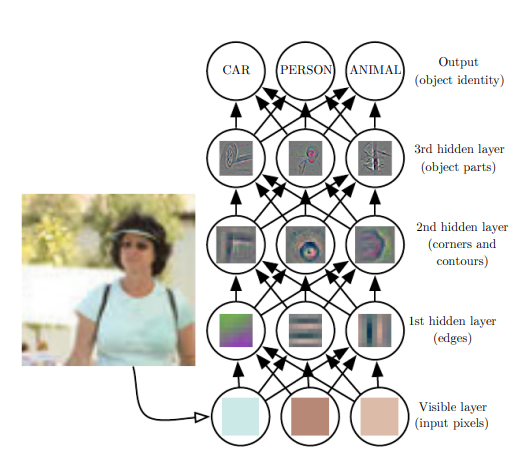
\includegraphics[width=0.5\linewidth]{deep_network}
	\caption{Schemat wielowarstwowej sieci neuronowej $\pagenote{Ian Goodfellow, Yoshua Bengio, Aaron Couville, \textit{Deep Learning Systemy uczące się}, PWN, Warszawa 2018}$}
	\label{fig:deepnetwork}
\end{figure}

Taka architektura została zaproponowana, ponieważ komputer nie potrafi zrozumieć znaczenia surowych danych reprezentowanych jako zbiór pikseli. Początkowe dane trafiają do widocznej warstwy początkowej, następnie warstwy ukryte wyciągają z obrazu cechy. Mając zbiór pikseli pierwsza warstwa ukryta może zidentyfikować krawędzie na podstawie porównań jasności sąsiednich pikseli. Kolejna warstwa, która zna krawędzie występujące na obrazku może zidentyfikować narożniki i rozszerzone kontury. Kolejna warstwa mając opisy z poprzednich warstw może wykryć całe fragmenty określonych obiektów. Opis obrazu w postaci kategorii: krawędzie, narożniki, obiekty i części może być wykorzystany do rozpoznania obiektów znajdujących się na obrazie. Podobny model można zastosować w przypadku generowania muzyki bądź wykrywania gatunku muzycznego na podstawie utworu. Utwór muzyczny posiada wiele cech: metrum, wysokość dźwięku, długość dźwięku. W takim przypadku każda warstwa sieci neuronowej może być odpowiedzialna za charakteryzację każdej cechy.

\section{Model sztucznego neuronu}

Sieci neuronowe nie są nową technologią. Pierwsze pomysły aby wykorzystać zasadzę działania ludzkich neuronów w modelach matematycznych pojawiły się w latach 40 ubiegłego wieku. Biologiczny neuron jest aktywowany na podstawie danych wejściowych. Dane pochodzą z kilku powiązanych neuronów wejściowych. Neurony za pomocą dendrytów rejestrują pozytywne i negatywne informacje wyjściowe z innych neuronów i kodują je za pomocą impulsów elektrycznych przesyłanych przez akson. Następnie akson rozdziela się i dociera do setek tysięcy dendrytów innych neuronów. Pomiędzy aksonem, a wejściowymi dendrytami następnych neuronów znajduje się synapsa. Synapsa odpowiada za przekształcanie impulsów elektrycznych na chemiczne sygnały wpływające na dendryt następnego neuronu. Wynik uczenia jest kodowany przez same neurony. Neurony przesyłają wiadomości aksonami wtedy, gdy poziom pobudzenia jest wystarczająco wysoki. 
\begin{figure}[H]
	\centering
	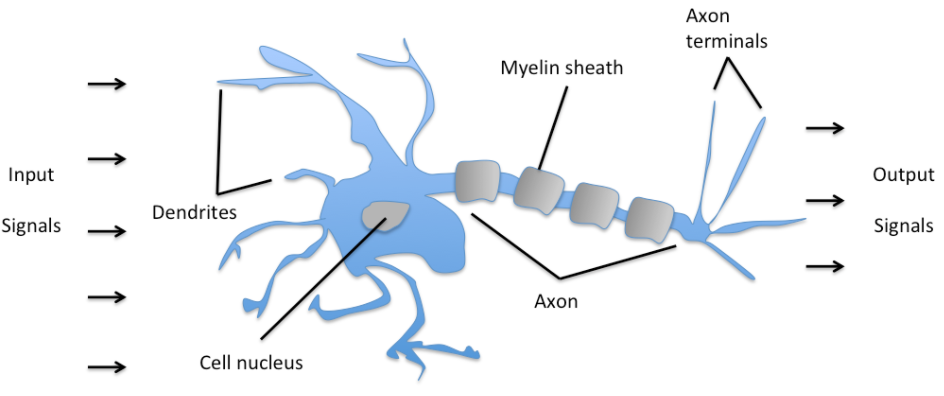
\includegraphics[width=0.7\linewidth]{schemat_neuronu}
	\caption{Schemat biologicznego neuronu \pagenote{\texttt{https://sebastianraschka.com/Articles/2015\_singlelayer\_neurons.html}}}
	\label{fig:schematneuronu}
\end{figure}

Warren McCulloch i Walter Pitts w roku 1943 opracowali model sztucznego neuronu, nazwali go $\textbf{MCP}$ od McCullock-Pitts$\pagenote{W. S. McCulloch and W. Pitts. A logical calculus of the ideas immanent in nervous activity. The bulletin of mathematical biophysics, 5(4):115–133, 1943}$ swoje wyniki opisali w dziele o nazwie \textit{A Logical Calculus of the Ideas Immanent in Nervous Activity}. Naukowcy przestawili neuron w postaci prostej bramki logicznej z binarnym wyjściem. Za pomocą neuronów MCP można zbudować prostą sieć neuronową, która realizuje funkcje logiczne AND i OR. Klika lat później w roku 1953 amerykański uczony Frank Rosenblatt zaproponował sztuczną sieć neuronową$\pagenote{F. Rosenblatt. The perceptron, a perceiving and recognizing automaton Project Para. Cornell Aeronautical Laboratory, 1957}$, którą nazwał perceptronem. Sieć zaprojektowana przez Rosenblatta mogła nauczyć się rozpoznawania ograniczonej klasy wzorców. Algorytm uczenia perceptronu polega na doborze wag dla sygnałów wejściowych w celu narysowania liniowej granicy decyzji, która pozwala nam rozróżnić dwie liniowo rozłączne klasy. Dane wejściowe są otrzymywane za pośrednictwem odpowiedników dendrytów, następnie obliczana jest suma z uwzględnieniem wag. Jeżeli dane wyjściowe przekroczą określony próg, a wejście hamujące nie jest aktywne to neuron wygeneruje wartość pozytywną. Jeżeli wejście hamujące jest aktywne, dane wyjściowe są hamowane, oznacza to że dane są niepoprawne. Model sztucznego neuronu jest modelem liniowym w przestrzeni n-wymiarowej gdzie n to liczba wejść neuronu, a wejścia powiązane są ze współczynnikami. 

\begin{figure}[H]
	\centering
	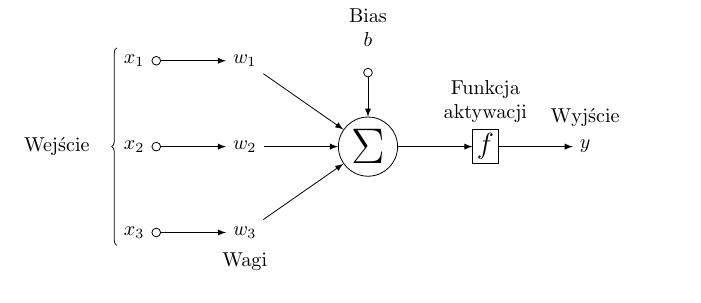
\includegraphics[width=0.5\linewidth]{perceptron_latex}
	\caption{Model perceptronu}
	\label{fig:neuron}
\end{figure}

Wejście $a$ można opisać za pomocą równania $a = w_{1}x_{1} + ... + w_{m}x_{n}$, gdzie:

\[
\textbf{w} = 
\begin{bmatrix}
w_{1} \\ \dots \\ w_{n}
\end{bmatrix},
 \textbf{x} =
\begin{bmatrix}
x_{1} \\  \dots \\ x_{n}
\end{bmatrix}
\]

Mając zdefiniowany wektor wejść oraz wag powyższe równanie można rozszerzyć do:

\begin{gather*} 
a = w_{0}x_{0} + w_{1}x_{1} + ... + w_{n}x_{n} = \textbf{w}^{T}\textbf{x}
\end{gather*}



Opis modelu:
\begin{itemize}
	\item Każde wejście $x_{n}$ posiada wagę $w_{n}$. Wartość wejścia jest mnożona przez wartość wagi.
	\item Obliczana jest suma $\sum w_{i}x_{i}$
	\item Funkcja aktywacji $\phi(a)$ pobudza neuron w zależności od zwróconej wartości (większej od granicy $\theta$ lub nie).
\end{itemize}

Prościej, model sztucznego neuronu można opisać za pomocą dwóch równań:
\begin{itemize}
	\item $a  = \sum_{j=1}^{n} w_{j}x_{j}$
	\item $y  = \phi (u + w_{0}) $
\end{itemize}

Funkcja aktywacji $\phi$ jest funkcją progową, to znaczy, że wyjście funkcji jest równe 1 dla dowolnej wartości wejściowej nie większej niż $\theta$.


\[
\phi(a)= 
\begin{cases}
1, & \text{if }  a \geq \theta \\
-1,              & \text{w przeciwnym wypadku}
\end{cases}
\]

Model perceptronu ma trzy ważne cechy:
\begin{itemize}

\item	Do sumy dodawany jest błąd systematyczny (ang. bias) uwzględniany przy sprawdzaniu progu. Ma to kilka celów. Po pierwsze, pozwala uwzględnić błąd statystyczny występujący w neuronach wejściowych. Po drugie, umożliwia standaryzację progów z użyciem wartości (na przykład zera) bez utraty ogólności.

\item	W perceptronie wagi wartości wejściowych mogę być niezależne od siebie i ujemne. Oznacza to dwie ważne rzeczy. Po pierwsze, neuronu nie trzeba wielokrotnie wiązać z wejściem, aby zwiększyć znaczenie danego wejścia. Po drugie, wejście z dendrytu może mieć wpływ hamujący, jeśli przypisana jest mu ujemna waga.

\item	Opracowanie perceptronu dało początek algorytmom uczącym się optymalnych wag na podstawie zbioru danych wejściowych i wyjściowych
\end{itemize}


\subsubsection{Algorytm uczenia się Perceptronu}   

\begin{enumerate}
	\item  Stwórz wektor wag składający się z liczb z przedziału 0, 1
	\item  Dla każdej wartości treningowej $x^{(i)}$:
		\begin{enumerate} 
			\item Oblicz wartość wyjściową $ \hat{y} $
			\item Zaktualizuj wag
			\end{enumerate}
\end{enumerate}

Wartość wyjściowa $\hat{y}$ to etykieta klasy do której zostało przyporządkowane dane wejście. Aktualizację każdej wagi $w_{j}$ w wektorze wag $\textbf{w}$ można zapisać jako:


\begin{gather*} 
w_{j} := w_{j} + \Delta w_{j}
\end{gather*}

Wartość $\Delta w_{j}$, która służy do aktualizacji wag obliczana jest według tak zwanej reguły uczenia perceptronu:

\begin{gather*} 
\Delta w_{j} = \eta ( y^{(i)} - \hat{y}^{(i)} ) x_{j}^{(i)}
\end{gather*}

Gdzie $\eta$ to pewna stała uczenia, zwykle wybierana z przedziału pomiędzy 0, 1. $y^{(i)}$ jest etykietą  i-tej próbki szkoleniowej, a $\hat{y}^{(i)}$ jest przewidywaną etykietą klasy. Wszystkie wagi w wektorze wagowym są aktualizowane jednocześnie. 

\begin{definicja}
	Proces uczenia neuronu wymaga zdefiniowania hipotezy $h_{\theta}$. Dla danych wejściowych $x^{(i)}$ predykcje można opisać za pomocą $h_{\theta}(x^(i))$
\end{definicja}

\begin{definicja} 
	Funkcja straty:
	 \begin{equation}
		  L:(z,y) \in \mathbb{R} \times Y \rightarrow L(z,y) \in \mathbb{R}
	 \end{equation}
	  Funkcja przyjmuje dane wejściowe $z$ oraz ich przewidywaną wartość $y$. Funkcja zwraca liczbę mówiącą o tym jak bardzo dane $z$ oraz $y$ różnią się między sobą.
\end{definicja}

\begin{definicja}
	Funkcja kosztu $J$ jest używana do zebrania informacji na temat efektywności procesu uczenia się. Do jej zdefiniowana używana jest funkcja straty $L$.
	\begin{equation}
		J(\theta) = \sum_{i=1}^{m} L(h_{\theta} (x^{(i)}), y^{(i)})
	\end{equation}
	W uczeniu nadzorowanym występują różne funkcje kosztu. Zostały one pokazane w tabeli poniżej.
	\newline
	\begin{table}[H]
	\bgroup
	\def\arraystretch{1.5}
	\captionof{table}{Zestawienie funkcji kosztu} 
	\centering
	\begin{tabular}{|c|c|c|c|}
		\hline 
		MSE& Strata logistyczna & Utrata zawiasów & Entropia krzyżowa \\ 
		\hline 
		$\frac{1}{2} (y - z)^{2}$ & $log(1 + exp(-yz))$ & $max(0,1 - yz)$ & $- \big[ylog(z) + (1-y)log(1-z) \big] $ \\ 
		\hline 
		 Regresja liniowa&Regresja logistyczna & SVM & Sieci neuronowe  \\ 
		\hline 
	\end{tabular} 
	\egroup
	\end{table}

	Jeżeli funkcja kosztu $J$ jest różniczkowalna do jej minimalizacji można użyć metody największego spadku gradientowego. Celem metody spadku gradientowego jest znalezienie takich wag, które minimalizują funkcję kosztu. Wartość $\frac{1}{2}$ na początku wzoru dodana jest dla ułatwienia obliczeń.
	
\end{definicja}

\begin{twierdzenie}
	Uczenie sieci neuronowej polega na minimalizacji funkcji kosztu.
\end{twierdzenie}

\begin{twierdzenie}
	Jeśli zbiór danych jest liniowo separowalny, a współczynnik szybkości uczenia $ \eta $ jest wystarczająco mały to algorytm uczenia perceptronu jest zbieżny.
\end{twierdzenie}

\begin{twierdzenie}
	Jeśli zbiór danych nie jest liniowo separowalny to algorytm zbiega lokalnie do minimalnego błędu średniokwadratowego.
\end{twierdzenie}


\section{Metoda spadku gradientowego}

Celem algorytmu spadku gradientowego jest minimalizacja funkcji kosztu $J(w)$. Minimalizacja funkcji kosztu pozwala na odpowiedni dobór wag. Ogólnie mówiąc minimalizacja funkcji polega na schodzeniu po jej powierzchni w oparciu o jej nachylenie. Aktualizacja wag polega na wykonaniu kroku w kierunku przeciwnym do gradientu $\nabla J(w)$ funkcji kosztu $J(w)$.
\begin{gather*} 
w := w + \Delta w
\end{gather*}

Gdzie zmiana wagi $\Delta w$ zdefiniowana jest jako:
\begin{gather*} 
\Delta w = - \eta \nabla J(w)
\end{gather*}

gdzie $\eta$ to stała uczenia - szybkość schodzenia w dół. Aby obliczyć gradient funkcji kosztu potrzeba wyliczyć pochodną cząstkową funkcji kosztu dla danej wagi $w_{j}$:

\begin{equation}
\frac{\partial J}{\partial w_{j}} = - \sum ( y^{(i)} - \phi(z^{(i)})) x_{j}^{(i)}
\end{equation}

Zatem reguła aktualizacji wag może wyglądać w następujący sposób:

\begin{equation}
	 \delta w_{j} = -\eta \frac{\partial J}{\partial w_{j}} = \eta \sum_{i} ( y^{(i)} - \phi(z^{(i)})) x_{j}^{(i)}
\end{equation}

\begin{przyklad}
	Dana jest funkcja jednej zmiennej $ y = f(x) = x^{2} - 4x + 2$, funkcja jest ciągła więc do znalezienia jej globalnego minimum można użyć algorytmu spadku gradientowego, rezultat został pokazany poniżej.
	\begin{figure}[H]
		\centering
		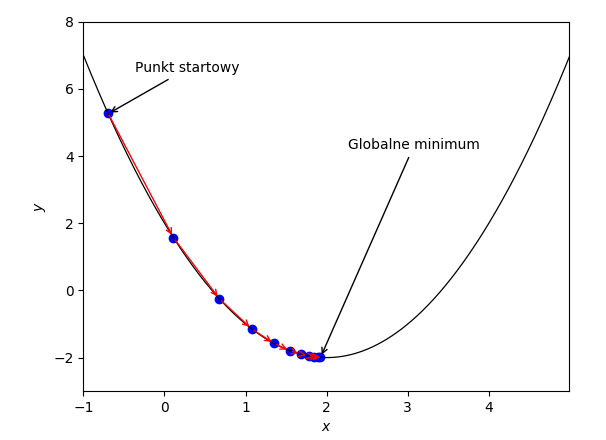
\includegraphics[width=0.5\linewidth]{gradient}
		\caption{Metoda spadku gradientowego}
		\label{fig:gradient}
	\end{figure}

	Poniżej wynik działania algorytmu za dużą stałą uczenia $\eta$:
	\begin{figure}[H]
		\centering
		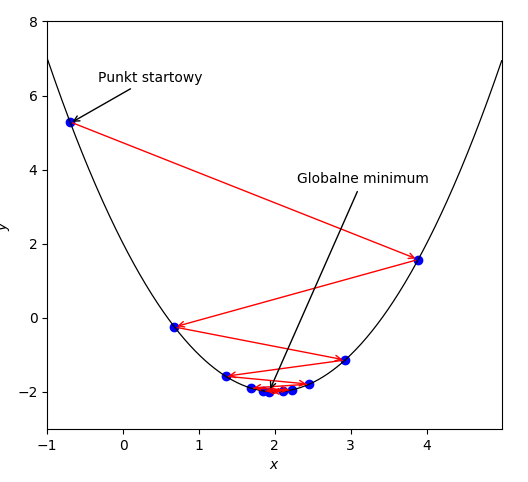
\includegraphics[width=0.5\linewidth]{gradient_wysoki_eta}
		\caption{Za duży współczynnik uczenia}
		\label{fig:gradientwysokieta}
	\end{figure}
	

\end{przyklad}

\begin{przyklad}
	Funkcję wielu zmiennych można również minimalizować za pomocą spadku gradientowego, pod warunkiem, że taka funkcja jest ciągła. Wyniki można obserwować na płaszczyźnie 3D.
\end{przyklad}

\begin{figure}[H]
	\centering
	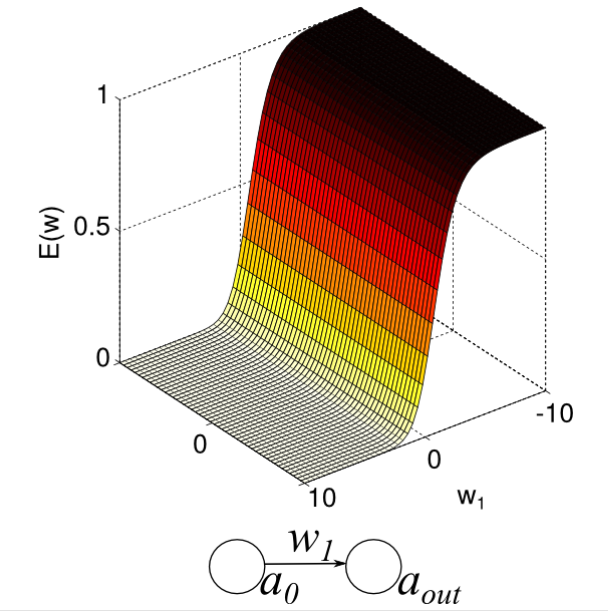
\includegraphics[width=0.4\linewidth]{1layererror}
	\caption{Przestrzeń błędów dla sieci jednowarstwowej}
	\label{fig:1layererror}
\end{figure}

\begin{figure}[H]
	\centering
	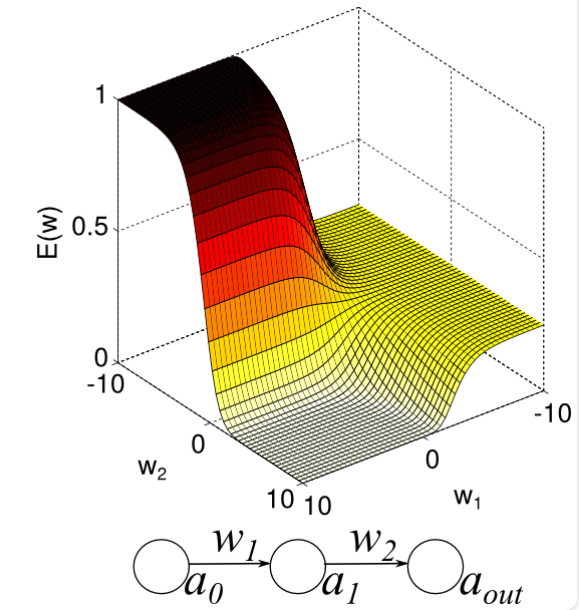
\includegraphics[width=0.4\linewidth]{2layererror}
	\caption{Przestrzeń błędów dla sieci dwuwarstwowej}
	\label{fig:2layererror}
\end{figure}



\section{Wielowarstwowe sieci neuronowe}

Sieci, które składają się przynajmniej z dwóch neuronów muszą mieć określoną architekturę, ponieważ wyniki zwracane przez te neurony mogą być wejściami dla innych neuronów. Takie sieci można podzielić na dwa rodzaje:
\begin{itemize}
	\item skierowane (ang. feed-forward)
	\item rekurencyjne (ang. recurrent)
\end{itemize}

W sieciach wielowarstwowych wyróżnia się podzbiór neuronów akceptujący dane wejściowe, nazywa się je jednostkami wejściowymi oraz podzbiór neuronów, których wyjście jest również wyjściem całej sieci, są to jednostki wyjściowe. Pozostałe neurony nazywa się ukrytymi. Sieci wielowarstwowe są w stanie przeprowadzić nieliniowy podział danych. Dane wejściowe każdej warstwy pochodzą z warstwy poprzedniej, a dane wejściowe poszczególnych warstw są danymi wejściowymi dla warstw następnych. Sieci skierowane są nazywane również sieciami jednokierunkowymi ponieważ związane to jest z tym, że dane płyną tylko w jedną stronę sieci, nie występują w niej cykle. Sieć wielowarstwową można powiązać ze skierowanym grafem acyklicznym opisującym, jak funkcje są ze sobą powiązane. Załóżmy sytuacje, w której mamy trzy funkcje $f^{(1)}, f^{(2)} i f^{(3)}$ połączone w łańcuch, tworząc $f(x) = f^{(3)} (f^{(2)} ( f^{(1)} (x)))$. Sieci wielowarstwowe najczęściej reprezentuje się właśnie w postaci takich struktur łańcuchowych. W takiej strukturze mówimy, że $f^{(1)}$ jest pierwszą warstwą sieci, $f^{(2)}$ to druga warstwa sieci. Całkowita długość łańcucha funkcji daje w wyniki głębokość modelu. Poniżej został przedstawiony model wielowarstwowej sieci neuronowej, który zawiera $(L+1)$-warstw z $D$ wejściami oraz $C$ wyjściami.


\begin{figure}[H]
	\centering
	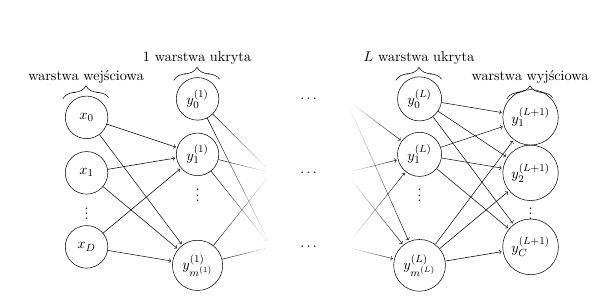
\includegraphics[width=0.7\linewidth]{multi_layer_neural}
	\caption{Model wielowarstwowej sieci neuronowej}
	\label{fig:multilayerneural}
\end{figure}



Wagę wielowarstwowych sieci neuronowych pokazują następujące ważne twierdzenia:

\begin{twierdzenie}
	Każda funkcja boolowska może być reprezentowana przez sieć z jedną warstwą ukrytą, ale może wymagać wykładniczej liczby jednostek ukrytych.
\end{twierdzenie}

\begin{twierdzenie}
	Każda ograniczona funkcja ciągła może być aproksymowana z dowolnie małym błędem przez sieć z jedną warstwą ukrytą [Cybenko1989; Hornik et al. 1989]
\end{twierdzenie}

\begin{twierdzenie}
	Dowolna funkcja może być aproksymowana z dowolną dokładnością przez sieć z dwoma warstwami ukrytymi [Cybenko 1988]
\end{twierdzenie}

Sieć neuronowa złożona z jednej warstwy ma ograniczenia, ponieważ może tylko realizować problemy liniowo separowalne. Bardzo klasycznym nieliniowym problemem jest funkcja XOR (alternatywa wykluczająca). Funkcja działa na dwóch wartościach bitowych $x_{1}$ i $x_{2}$. Funkcja zwraca 1 wtedy gdy dokładnie jedna z dwóch wartości jest równa 1. Ograniczenia sieci jednowarstwowych opisali Marvin Minsky i Seymour Papert w książce po tytułem Perceptrons: An Introduction to Computational Geometry. W swojej książce przedstawili funkcję XOR jako problem nieliniowy, z którym pojedynczy perceptron lub jednowarstwowa sieć sobie nie poradzi. 

 
	\begin{table}[H]
	\centering
	\begin{tabular}{@{ }c@{ }@{ }c | c@{ }@{ }c@{ }@{ }c@{ }@{ }c@{ }@{ }c}
		p & q &  & p & XOR & q & \\
		\hline 
		0 & 0 &  &  &  0& \\
		0 & 1 &  &  &  1 & \\
		1 & 0 &  & &   1& \\
		1 & 1 &  &  & 0& \\
	\end{tabular}
	\caption{Tabela prawdy dla funkcji XOR} \label{tab:sometab}
	\end{table}
 

Funkcja XOR przedstawiona na wykresie dowodzi, że jej dane wyjściowe nie są liniowo separowalne w przestrzeni dwuwymiarowej. To znaczy, że nie istnieje jedna prosta, która pozwalałaby na rozdzielenie elementów klasy pozytywnej i negatywnej. Punkty można poprawnie rozdzielić przy pomocy więcej niż jednej prostej. Taką możliwość daje architektura sieci wielowarstwowej. Aby skonstruować sieć, która będzie wstanie nauczyć się problemu XOR wystarczy sieć dwuwarstwowa z jedną warstwą ukrytą. Sieć na wejściu przyjmuje dwie wartości, które potrzebne są do obliczenia funkcji XOR. W tak opracowanej sieci każdy węzeł tworzy hiperpłaszczyznę. Wszystkie hiperpłaszczyzny są łączone przez końcowy perceptron. W efekcie otrzymujemy podprzestrzeń, która jest zbiorem wypukłym. Kolejnym ważnym problemem jest odpowiedni dobór wag, które trzeba wyliczyć automatycznie. Wagi powinny być tak dobrane aby można było je wykorzystać do klasyfikowania i prognozowania danych innych niż te pierwotne wejściowe. 

\section{Funkcje aktywacji}

Sieci neuronowe pozwalają na stosowanie szerokiego zakresu funkcji aktywacji. Wybór funkcji aktywacji zależy głównie od tego jaki problem sieć neuronowa powinna rozwiązać. W sieciach wielowarstwowych najczęściej stosowane są funkcje nieliniowe, ponieważ ich nieliniowość jest ważną cechą potrzebną do sprawnego uczenia. Funkcje aktywacje można podzielić na:

\begin{itemize}
	\item nieliniowe
	\item liniowe
	\item skoku jednostkowego (progowa)
\end{itemize}

Ostatni rodzaj funkcji aktywacji jest najbardziej podstawową aktywacji neuronu. Funkcja ta umożliwia otrzymanie na wyjściu sieci informacji postaci TAK - NIE. 

\begin{equation}
f(x)= 
\begin{cases}
0,&  x < 0\\
1,   & x \ge 0
\end{cases}
\end{equation}

\begin{figure}[H]
	\centering
	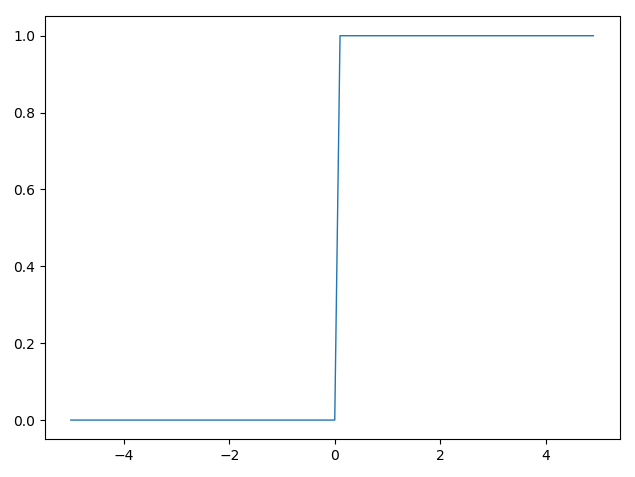
\includegraphics[width=0.5\linewidth]{stepfunction}
	\caption{Funkcja skoku jednostkowego}
	\label{fig:stepfunction}
\end{figure}

Jeżeli sieć neuronowa ma spełniać zadanie klasyfikatora binarnego (zwraca TAK lub NIE), to funkcja progowa będzie idealną funkcją aktywacji. Problem może pojawić się jeżeli będziemy chcieli wprowadzić więcej klas klasyfikacji. Wtedy jeżeli więcej niż jeden neuron zostanie aktywowany to reszta neuronów automatycznie wyprowadzi 1 z funkcji progowej. Dla większej ilości klas byłoby lepiej, gdy funkcja aktywacji nie była binarna tylko zwracała wartości w postaci np. 20\% dla jednej klasy 50\% dla drugiej i reszta dla ostatniej.

\subsection{Funkcja liniowa}

W przypadku funkcji liniowej sygnał wyjściowy przyjmuje postać:

\begin{equation}
y = cx
\end{equation}

\begin{figure}[H]
	\centering
	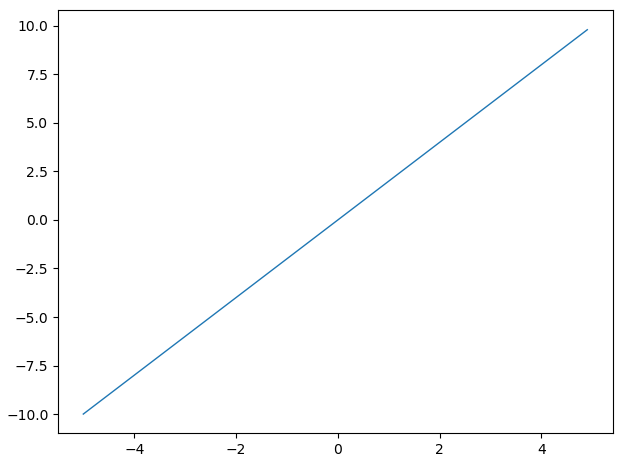
\includegraphics[width=0.5\linewidth]{funkcjaLiniowa}
	\caption{Funkcja liniowa}
	\label{fig:funkcjaliniowa}
\end{figure}

W przypadku liniowej funkcji aktywacji aktywacja jest proporcjonalna do sygnału wejściowego neuronu (który jest sumą ważoną).
Takie podejście daje szereg różnych aktywacji, nie ma w tym przypadku aktywacji binarnej. Przy treningu neuronu z liniową funkcją aktywacji może wystąpić problem, ponieważ pochodna dla tej funkcji jest stała. Oznacza to, że gradient nie ma związku z $x$. Jeżeli gradient jest stały to metoda spadku gradientowego również zwróci stały gradient. Jeżeli zostanie użyta wsteczna propagacja błędu to zmiany wprowadzone przez algorytm również będą stałe i nie będą zależne od zmiany wejścia. Bez względu na to z ilu warstw jest zbudowana sieć neuronowa to ostatnia funkcja aktywacji w ostatniej warstwie jest liniową funkcją wejścia pierwszej warstwy.

\subsection{Funkcja sigmoidalna i tanh}

Popularną nieliniową funkcją aktywacji jest funkcja sigmoidalna, której kształt przypomina literę $S$.

\begin{equation}
	f(x) = \frac{1}{1 + e^{-x}}
\end{equation}

\begin{figure}[H]
	\centering
	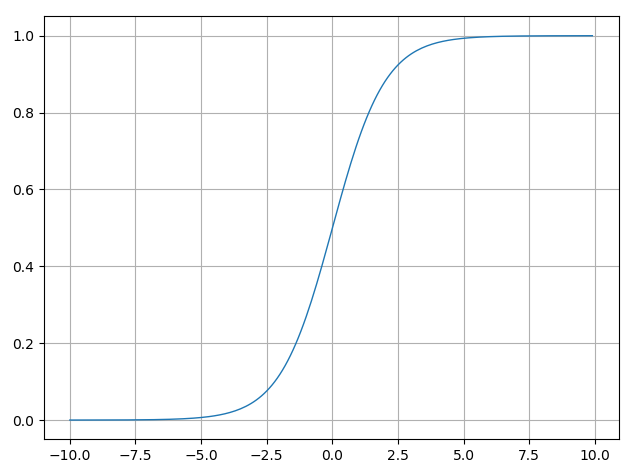
\includegraphics[width=0.5\linewidth]{sigmoid}
	\caption{Wykres funkcji sigmoidalnej}
	\label{fig:sigmoid}
\end{figure}

Bardzo ważną cechą funkcji sigmoidalnej jest fakt, że jest różnoczkowalna. Warto zauważyć, że pomiędzy wartościami -2 do 2 wartości z osi $y$ są bardzo strome. Każda niewielka zmiana wartości $x$ w tym regionie spowoduje znaczne zmiany wartości $y$. Ten fakt można wykorzystać do doprowadzania wartości $y$ do jednego z końców krzywej. Wyjście funkcji zawsze będzie znajdować się w zakresie $(0, 1)$. W przypadku gdy wartości zwracane przez funkcją będą bardzo blisko krańców krzywej to gradient będzie bardzo mały, na tyle mały że nie będzie można dokonać zmiany wag. W takim przypadku może dojść do sytuacji, że sieć nie będzie w stanie się uczyć lub proces uczenia będzie bardzo wolny. Taki problem określa się mianem znikającego gradientu$\pagenote{\texttt{https://arxiv.org/pdf/1211.5063.pdf}}$.

\\

Kolejną używaną funkcją aktywacji w sieciach neuronowych jest funkcja $\textit{tanh}$:

\begin{equation}
f(x) = tanh(x) = \dfrac{2}{1 + e^{-2x}} - 1
\end{equation}

powyższe równanie można sprowadzić do wcześniej wspomnianej funkcji sigmoidalnej:

\begin{equation}
tanh(x) = 2sigmoid(2x) - 1
\end{equation}

\begin{figure}[H]
	\centering
	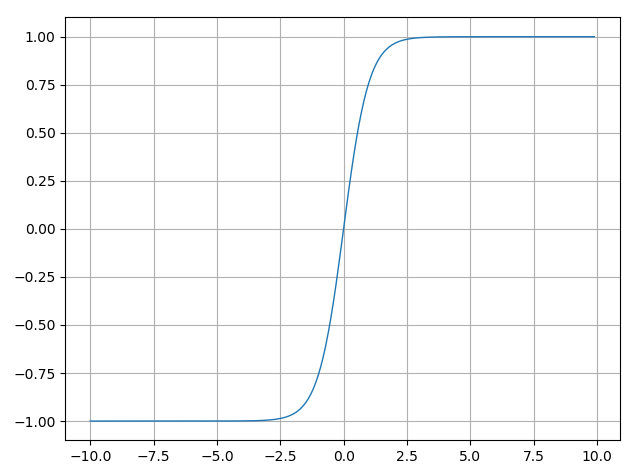
\includegraphics[width=0.5\linewidth]{tanh}
	\caption{Wykres funkcji tanh}
	\label{fig:tanh}
\end{figure}

Charakterystyka funkcji $tanh$ jest podobna jak w przypadku funkcji sigmoidalnej. W przypadku funkcji tanh gradient jest znacznie silniejszy niż w przypadku funkcji sigmoidalnej. Również w przypadku funkcji than występuje problem znikającego gradientu. 

\subsection{Funkcja ReLu}

\begin{equation}
	f(x) = max(0, x)
\end{equation}

Funkcja $\textit{Rectified Linear Units}$ jest zalecana do zastosowania w większości jednokierunkowych sieci neuronowych.

\begin{figure}[H]
	\centering
	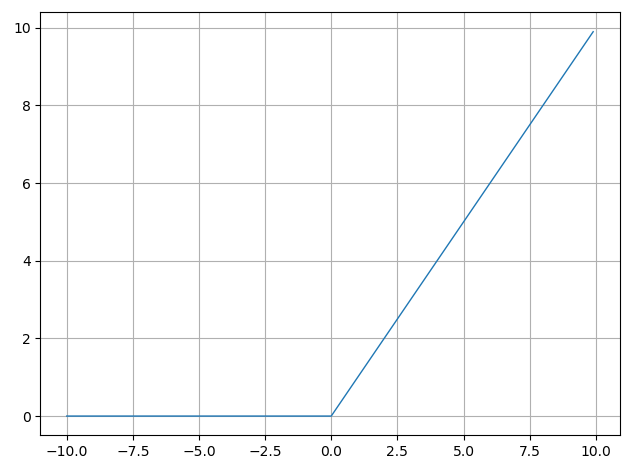
\includegraphics[width=0.5\linewidth]{relu}
	\caption{Funkcja ReLu}
	\label{fig:relu}
\end{figure}

Funkcja $ReLu$ jest funkcją nieliniową, która zwraca wartości z przedziału $<0, \infty$. Z wykresu funkcji można odczytać, że funkcja $ReLu$ może rzadko aktywować neuron. Dla ujemnych wartości $x$ funkcja zwraca wartość 0, co wyraźnie widać na wykresie w postaci poziomej linii. W przypadku aktywacji ten obszar funkcji $ReLu$ dla gradientu będzie wynosił 0. Oznacza to, że neurony wchodzące w ten obszar przestaną reagować na zmiany. O tym zjawisku mówi się jako o "umieraniu neuronu" lub "problem umierającego ReLu". Ten problem może spowodować sytuacje, że kilka neuronów po prostu umrze i nie będzie reagować przez co część sieci do niczego się nie przyda. Funkcja $ReLu$ jest znacznie mniej kosztowna obliczeniowo niż $tanh$ i $sigmoid$. Warto ja rozważyć w przypadku projektowania głębokiej sieci neuronowej. 

Podsumowując, wymagane cechy funkcji aktywacji to:
\begin{itemize}
	\item ciągłe przejście pomiędzy swoją wartością maksymalną a minimalną (funkcja musi być ciągła)
	\item łatwa do obliczenia i ciągła pochodna
\end{itemize} 


\section{Wsteczna propagacja błędu}

W sieciach jednokierunkowych gdzie na wejściu przyjmowany jest wektor $x$ dane wejściowe podają początkową informację, która przepływa w górę do ukrytych jednostek w każdej sieci, w rezultacie otrzymujemy $\hat{y}$. Jedną z głównych zalet sieci neuronowych jest to, że nie musimy ręcznie podawać wag. Można te wagi wytrenować, czyli znaleźć ich w przybliżeniu optymalny zestaw za pomocą algorytmu wstecznej propagacji błędu. Autorami algorytmu są D. E. Rumelhart, G. E. Hinton,
i R. J. Williams, swoje wyniki opublikowali na łamach prestiżowego magazynu $\textit{Nature} \pagenote{Learning representations by back-propagating errors, D. E. Rumelhart, G. E. Hinton,
	and R. J. Williams, Nature, 323: 6088, strony 533–536, 1986}$  Po mimo tego, że sam algorytm ma ponad 30 lat to jest jednym z najważniejszych algorytmów stosowanych do efektywnego uczenia sieci neuronowych. O samym algorytmie można myśleć jak o wydajnej metodzie, która służy do obliczania pochodnych cząstkowych funkcji kosztu w wielowarstwowych sieciach neuronowych. Problem w wielowarstwowych sieciach polega na tym, że mamy do czynienia z bardzo dużą liczbą współczynników, które trzeba wyznaczyć. W przeciwieństwie do pozostałych modeli funkcja kosztu w sieci wielowarstwowej nie jest wypukła ani gładka w odniesieniu do parametrów. Istnieje więc wiele nierówności w wielowymiarowej przestrzeni, które trzeba zoptymalizować tak aby znaleźć globalne minimum. W algorytmie wstecznej propagacji błędów jest wykorzystywana reguła łańcuchowa, której zadaniem jest obliczenie pochodnej funkcji złożonej.

\begin{fact}
	Algorytm propagacji wstecznej działa dla dowolnego grafu skierowanego bez cykli.
\end{fact}

\begin{twierdzenie}
	Algorytm propagacji wstecznej zbiega lokalnie do minimalnego błędu średniokwadratowego.
\end{twierdzenie}


\begin{equation}
\frac{d}{dx}
\big[ f(g(x)) \big] = \frac{df}{dg} \cdot \frac{dg}{dx}
\end{equation}

	Reguły łańcuchowej możemy użyć do długiej złożonej funkcji, funkcja ta może reprezentować wielowarstwową sieć neuronową. Załóżmy, że sieć składa się z pięciu warstw: $F(x)= f(g(g(u(v(x)))))$. Po zastosowaniu reguły łańcuchowej możemy policzyć pochodne ze wzoru:
	
	\begin{equation}
		\frac{dF}{dx} = \frac{d}{dx}F(x)=\frac{d}{dx}f(g(h(u(v(x))))) = \frac{df}{dg} \cdot \frac{dg}{dh} \cdot \frac{dh}{du} \cdot \frac{du}{dv} \cdot \frac{dv}{dx}
	\end{equation}
	
	W algorytmie wstecznej propagacji wykorzystuje się pochodną funkcji aktywacji. Pochodna informuje o tym czy dla zadanego zestawu wag funkcja aktywacji jest odpowiednio pobudzona. Dzięki temu można dowiedzieć się w którym kierunku i jak bardzo zaktualizować wagi.
	
	Poniżej zostanie przedstawiony proces uczenia wielowarstwowej sieci neuronowej z użyciem algorytmu wstecznej propagacji błędu na przykładzie trójwarstwowej sieci neuronowej o dwóch wejściach i jednym wyjściu. Przepływ w takiej sieci można wyrazić za pomocą listy kroków:
	
	\begin{itemize}
		\item Warstwa wejściowa $Z$  jest wyrażona za pomocą równania $Z = A * W$, gdzie $A$ to macierz danych wejściowych, a $W$ to macierz wag dla danych wejściowych
		\item Iloczyn oby macierzy trafia do funkcji aktywacji $A$, operację można wyrazić za pomocą wzoru $A = \phi(Z))$ - operacja odbywa się w warstwie ukrytej
		\item Wynik funkcji aktywacji trafia do warstwy wyjściowej i jest wymnażany przez macierz wag $Z = A * W$
		\item Obliczone dane w warstwie wyjściowej trafiają do funkcji aktywacji $A = \phi(Z)$, wynik przypisywany jest do $z$
	\end{itemize}

	W taki sposób została dokonana propagacja sygnału przez całą sieć w kierunku od lewej strony do prawej.	W algorytmie wstecznej propagacji błędu błąd jest propagowany z prawej do lewej. Proces zaczyna się od obliczenia błędu w warstwie wyjściowej:
	
	\begin{equation}
	\delta = z - y 
	\end{equation}
	
	Sygnał wyjściowy sieci porównywany jest z oczekiwaną wartością sygnału wyjściowego. Różnica obu wartości nazywana jest sygnałem błędu $\delta$ neuronu warstwy wyjściowej. Neurony, które znajdują się w warstwach ukrytych nie są w stanie bezpośrednio określić swojego błędu, ponieważ nie są znane wartości oczekiwane sygnałów wyjściowych z tych neuronów. Dzięki wstecznej propagacji błędu błąd jest rzutowany wstecz od prawej do lewej strony. Dzięki temu można obliczyć błąd w warstwie ukrytej.
	
	\begin{equation}
	\delta^{(hidden)} = \delta \big( W \big) ^{T} \frac{\partial \phi(Z^{(hidden)}))}{\partial Z ^{(hidden)}}
	\end{equation}
	
	uwzględniając pochodną funkcji aktywacji powyższe wyrażenie można zapisać jako:
	
	\begin{equation}
		\delta^{(hidden)} = \delta \big(W \big)^{T} \big(a^{(h)} \big(1-a^{(h)}\big)\big)
	\end{equation}
	
	W dalszej kolejności trzeba przechować pochodną cząstkową każdego węzła każdej warstwie oraz błąd węzła w następnej warstwie. Należy obliczyć $\delta_{i,j}^{(l)}$ dla każdej próbki ze zbioru treningowego.
	
	\begin{equation}
		\Delta ^{(hidden)} = \delta^{(hidden)} + \big(A^{(input)}\big)^{T} \delta^{(hidden)}
	\end{equation}
	
	\begin{equation}
	\Delta  = \delta + \big(A^{(hidden)}\big)^{T} \delta
	\end{equation}

	Po wyliczeniu spadku gradientowego należy zaktualizować wagi wykonując przeciwny kroku w kierunku gradientu dla każdej warstwy:
	
	\begin{equation}
		W^{(l)} := W^{(l)} - \eta \Delta^{(l)}
	\end{equation}

	Cały proces można przedstawić za pomocą ilustracji poniżej i przedstawić za pomocą listy kroków:
		
	\begin{figure}[H]
		\centering
		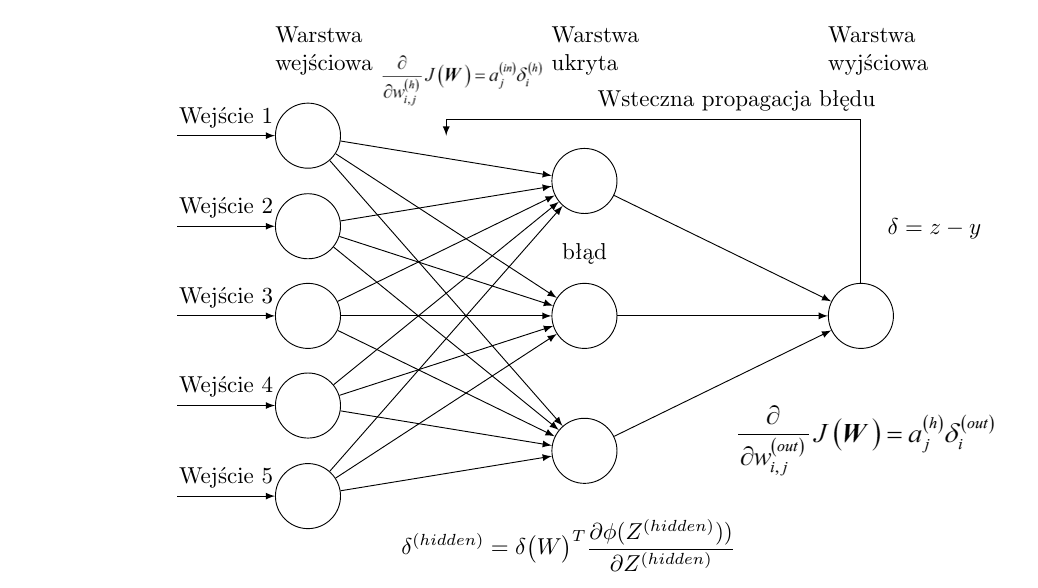
\includegraphics[width=0.9\linewidth]{backprop}
		\caption{Ilustracja wstecznej propagacji błędu}
		\label{fig:backprop.png}
	\end{figure}
	Cały proces można sprowadzić do listy kroków:
	\begin{itemize}
		\item Pobierz dane treningowe
		\item Przeprowadź propagacje sygnału w celu obliczenia błędu
		\item Przeprowadź propagację wsteczną aby uzyskać gradienty
		\item Użyj gradientów aby zaktualizować wagi sieci
	\end{itemize}


	\begin{fact}
	Zauważmy, że możemy określić pojęcie epoki jako jeden cykl podczas którego wszystkie obiekty treningowe poprawiają wagi, na koniec wyliczany jest błąd sumaryczny całego zbioru treningowego. Algorytm uczenia zatrzymuje się, kiedy błąd przestaje maleć.
	\end{fact}

	\begin{figure}[H]
		\centering
		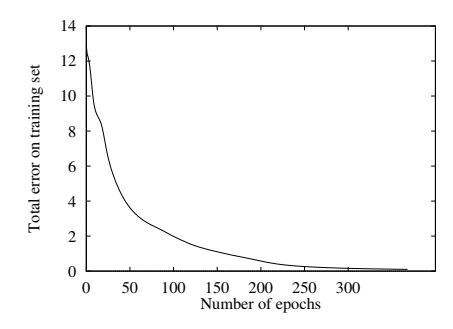
\includegraphics[width=0.7\linewidth]{epoki}
		\caption{Proces uczenia sieci polega na minimalizacji błędu}
		\label{fig:epoki}
	\end{figure}
	
	\section{Rekurencyjne sieci neuronowe}

	Rekurencyjne sieci neuronowe (ang. recurrent neural networks, RNN)(Rumenlhart 1986) to rodzina sieci neuronowych służąca do pracy z danymi sekwencyjnymi. Sieci rekurencyjne mają zastosowanie w tłumaczeniu tekstu, rozpoznawaniu obrazu, rozpoznawaniu mowy czy generowaniu muzyki, ponieważ wszystkie te mechanizmy potrzebują do działania sekwencji. Jedną z pierwszych koncepcji systemów uczących się i modeli statystycznych była możliwość współdzielenia parametrów w różnych częściach modelu. Takie podejście pozwala na rozszerzenie modelu i zastosowanie go do przykładów o różnych postaciach. Istnieje klika różnych kategorii przetwarzania danych sekwencyjnych, które można podzielić ze względu na dane wejściowe i wyjściowe. Takiego podziału dokonał Andrej Karpathy, który opisał w artykule \textit{The Unreasonable Effectiveness of Recurrent Neural Networks}\pagenote{\texttt{http://karpathy.github.io/2015/05/21/rnn-effectiveness/}} Rysunek poniżej obrazuje różne zależności między danymi wejściowymi, a wyjściowymi. 
	
	\begin{figure}[H]
		\centering
		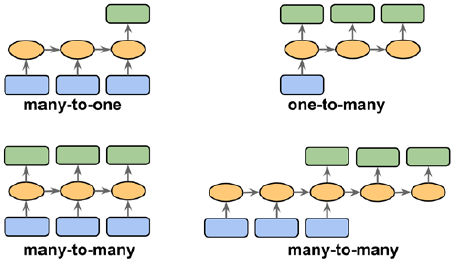
\includegraphics[width=0.7\linewidth]{relacje}
		\caption{Zależności pomiędzy wejściem, a wyjściem w rekurencyjnych sieciach neuronowych $\pagenote{Sebastian Raschka, \textit{Python Machine Learning}, Packt Publishing; 1 edition (September 23, 2015), 540}$}
		\label{fig:relacje}
	\end{figure}
	
	W przypadku kiedy dane wejściowe zawierają sekwencje istnieje klika różnych przypadków modeli, które to zwrócą różne wyjścia. Można je podzielić na trzy główne kategorie.
	
	
	\begin{itemize}
		\item Wiele do jednego - Dane wejściowe to sekwencja, wyjście to wektor o stałym rozmiarze. Dla przykładu na wejściu jest fragment tekstu, a na wyjściu jedno słowo np. emocja opisująca fragment tekstu, inny przykład to sekwencja nut na wejściu, a na wyjściu nazwa gatunku muzycznego pasującego do zadanej sekwencji.
		\item Jeden do wielu - Dane wejściowe nie są sekwencją, natomiast dane wyjściowe składają się z sekwencji. Przykład to opisywanie obrazów, wejście to obraz, a na wyjściu opis obrazu.
		\item Wiele do wielu - Dane wejściowe i wyjściowe składają się z sekwencji. Przykład to tłumaczenie jednego języka na inny, generowanie nowego utworu muzycznego na podstawie innego. 
	\end{itemize}

	W książce $\textit{Deep Learning}$ Yan Goodfellow dokonał podobnego podziału:
	
	\begin{itemize}
		\item sieci rekurencyjne, które generują wartości wynikowe w każdym kroku czasowym i mają rekurencyjne połączenia między ukrytymi jednostkami
		\item sieci rekurencyjne, które generują wartości wynikowe w każdym kroku czasowym i mają rekurencyjne połączenia jedynie między wejściem w jednym kroku czasowym, a jednostkami ukrytymi w kolejnym kroku czasowym
		\item sieci rekurencyjne z rekurencyjnymi połączeniami między ukrytymi jednostkami, które odczytują całą sekwencje, a następnie generują jedno wyjście
	\end{itemize}                 
	
		 Innym historycznym przykładem sieci rekurencyjnej jest sieci $\textbf{Elmana }$ (Elman, 1990) - sieć złożona z trzech podstawowych warstw (wejściowej, ukrytej, wyjściowej) oraz dodatkowej warstwy, której połączenia wejściowe są połączeniami wejściowymi warstwy ukrytej.
		 $\textbf{Sieci Jordana }$ posiadają podobną strukturę do sieci Elmana, połączenia wejściowe do warstwy kontekstowej są połączeniami wyjściowymi z warstwy wyjściowej.
		 $\textbf{Sieci Hopfielda }$ nie posiadają wyróżnionych warstw, każdy neuron połączony jest ze wszystkimi neuronami w sieci, poza sobą, neurony nie mają pętli, każda para neuronów ma połączenie symetryczne.

	Rekurencyjną sieć neuronową można przedstawić za pomocą poniższego wzoru, który oblicza sekwencje wektorów $x$ stosując zasadę rekurencji dla każdego kroku czasowego:
	
	\begin{equation}
	h_{t} = f_{W} ( h_{t-1}, x_{t} )
	\end{equation}
	
	\begin{itemize}
		\item $h_{t}$ - nowy stan
		\item $f_{W}$ - funkcja aktywacji z parametrem $W$
		\item $h_{t-1}$ - poprzedni stan
		\item $x_{t}$ - wektor wejścia w kroku czasowym $t$
	\end{itemize}
	
	Powyższy wzór można przedstawić za pomocą schematu:
	
	\begin{figure}[H]
		\centering
		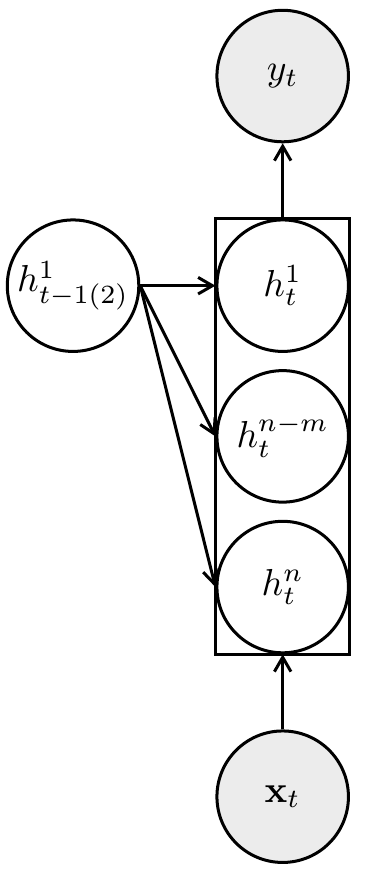
\includegraphics[width=0.2\linewidth]{rnn_model}
		\caption{Schemat rekurencyjnej sieci neuronowej z jedną warstwą ukrytą}
		\label{fig:rnn}
	\end{figure}
	
	Model sieci rekurencyjnej można rozwinąć w czasie, wtedy otrzymamy:
	
 	\begin{figure}[H]
 		\centering
 		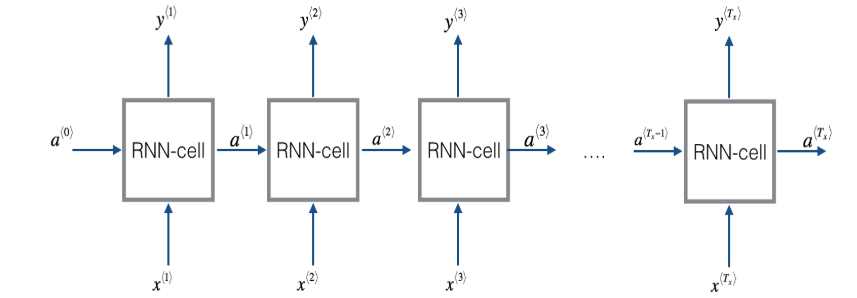
\includegraphics[width=0.7\linewidth]{rnn_forward_pass}
 		\caption{Rekurencyjna sieć neuronowa rozwinięta w czasie}
 		\label{fig:rnnforwardpass}
 	\end{figure}
 	
 	 Sekwencja wejściowa $x = (x^{1}, x^{2}, ..., x^{T_{x}})$ jest aplikowana do sieci w $T_{x}$ krokach czasowych. Na wyjściu sieć zwraca sekwencję $y = (y^{1}, y^{2}, ..., y^{T_{x}})$.
	
	Rekurencyjną sieć neuronową można postrzegać jako powtarzanie pojedynczej komórki. Poniższy rysunek opisuje operacje dla pojedynczego kroku czasowego komórki w rekurencyjnej sieci neuronowej.
	
	\begin{figure}[H]
		\centering
		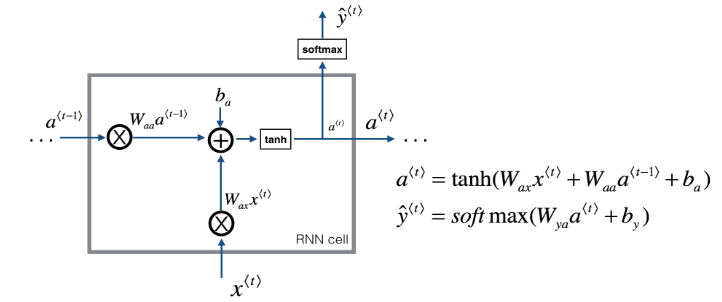
\includegraphics[width=0.7\linewidth]{rnn_cell}
		\caption{Podstawowa komórka w rekurencyjnej sieci neuronowej.}
		\label{fig:rnncell}
	\end{figure}

	 Powyższa komórka na wejściu otrzymuje $x^{t}$ oraz $a^{t-1}$ z poprzedniego ukrytego stanu, na wyjściu komórka zwraca $a^{t}$, wyjście będzie wykorzystane jako wejście do następnej komórki oraz zostanie użyte do predykcji $\hat{y}^{t}$

	Każda krawędź skojarzona jest z macierzą wag. Macierz wag jest niezależna od danego kroku czasowego $t$. Macierze wag, które występują na rysunku powyżej:
	
	\begin{itemize}
		\item $\textbf{\textit{W}}_{ax}$ - macierz wag pomnożona przez wektor wejściowy
		\item $\textbf{\textit{W}}_{aa}$ - macierz wag pomnożona przez stan ukryty
		\item $\textbf{\textit{W}}_{ya}$ - macierz wag pomiędzy warstwą ukrytą, a warstwą wyjściową
	\end{itemize} 
	
	Trening rekurencyjnej sieci neuronowej odbywa się z wykorzystaniem algorytmu \textit{Backpropagation Through Time}\pagenote{Backpropagation Through Time: What It Does and How to Do It (Paul Werbos, Proceedings of IEEE, 78(10):1550-1560, 1990).}. Algorytm bazuje na metodzie spadających gradientów. Jego główną ideą jest to aby całkowity błąd $L$ był sumą wszystkich funkcji błędu w czasie $t=1$ do $t=T$.

	\begin{equation}
		L = \sum_{t=1}^{T} L^{(t)}
	\end{equation}

	Sieci rekurencyjne stosuje się aby zachowywać długotrwałe zależności w czasie. Jednak niesie to ze sobą pewne problemy, ponieważ im więcej danych nagromadzonych w poszczególnych krokach czasowych to istnieje duże ryzyko, że gradienty obliczane z wykorzystaniem algorytmu BPTT będą się gromadzić. Takie zjawisko może doprowadzić do problemu zanikającego gradientu lub jego eksplozji. Problem ten został dokładnie opisany przez R. Pascanu, T. Mikolov, i Y. Bengio w dziele \textit{On the difficulty of training recurrent neural networks}\pagenote{\texttt{https://arxiv.org/pdf/1211.5063.pdf}}.
	
	Na przestrzeni lat zostały opracowane dwa sposoby, które rozwiązują ten problem:
	\begin{itemize}
		\item Truncated backpropagation through time (TBPTT)$\pagenote{\texttt{http://ir.hit.edu.cn/~jguo/docs/notes/bptt.pdf}}$ 
		\item Long short-term memory (LSTM)$\pagenote{\texttt{http://www.bioinf.jku.at/publications/older/2604.pdf}}$
	\end{itemize}
	\subsection{Pamięć Long Short-Term }
	Współcześnie najbardziej efektywne modele sekwencyjne, które stosowane są w praktyce nazywane są bramkowymi sieciami RNN. Do tych modeli zaliczana jest architektura długiej pamięci krótkoterminowej (ang. long short-term memory). Pierwsza koncepcja architektury LSTM została przedstawiona przez dwóch niemieckich naukowców S. Hochreiter'a oraz J. Schmidhuber'a w 1997 $\pagenote{Sepp Hochreiter, Jurgen Schmidhuber, \textit{Long Short-Term Memory}, Neural Computation}$. Głównym blokiem konstrukcyjnym LSTM jest komórka pamięci, która reprezentowana jest przez ukrytą warstwę w rekurencyjnej sieci neuronowej. Sieci rekurencyjne z blokiem LSTM nazywamy sieciami LSTM. Nad poprawieniem pierwotnej koncepcji LSTM pracowało wiele osób przez kilka lat, wyniki poprawek zostały opisane w pracy $\pagenote{In addition to the original authors, a lot of people contributed to the modern LSTM. A non-comprehensive list is: Felix Gers, Fred Cummins, Santiago Fernandez, Justin Bayer, Daan Wierstra, Julian Togelius, Faustino Gomez, Matteo Gagliolo, and Alex Graves.}$ Sieci LSTM zostały zaprojektowane w celu uniknięcia problemu długotrwałej zależności. Trening sieci LSTM pozwala na zapamiętanie długotrwałych zależności pomiędzy danymi wejściowymi, a wyjściowymi wynikami zwracanymi przez sieć. Struktura komórki LSTM może przypominać pamięć komputera, ponieważ może odczytywać, zapisywać i usuwać informacje za pomocą odpowiednich bramek. Komórka decyduje, czy przechować lub usunąć informacje w zależności od przypisanej wagi do informacji. Wagi dobierane są w procesie uczenia, z upływem czasu komórka LSTM dowiaduje się, które informacje są ważne, a które nie. Struktura komórki LSTM została przedstawiona na rysunku poniżej.
	
	\begin{figure}[H]
		\centering
		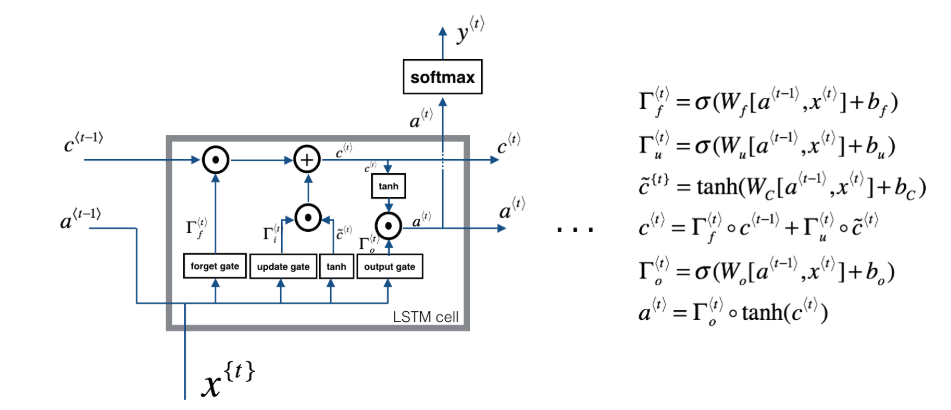
\includegraphics[width=1.0\linewidth]{lstm_cell}
		\caption{Komórka LSTM}
		\label{fig:lstmcell}
	\end{figure}
	Głównym rdzeniem komórki LSTM jest wyprowadzenie, które na wejściu przyjmuje pamięć z poprzedniego kroku czasowego $c^{\langle t-1 \rangle}$ i zwraca aktualny stan pamięci $c^{\langle t \rangle}$. Komórka posiada trzy wejścia. Pierwsze z nich to wektor $x^{t}$ w kroku czasowym $t$. $a^{\langle t-1 \rangle}$ oznacza wyjście z poprzedniej komórki LSTM. Wcześniej wspomniane $c^{\langle t-1 \rangle}$ to pamięć z poprzedniej jednostki. Symbol $\odot$ zamieszczony na schemacie to iloczyn Hadamarda.
	
	$\newline$
	Komórka LSTM posiada trzy różne typy bramek:
	
	\begin{itemize}
		\item Bramka zapomnienia (ang. forget gate) pozwala komórce pamięci na wymazanie pamięci. Wektory wejściowe po wymnożeniu przez wagi trafiają do sigmoidalnej funkcji aktywacji. Funkcja aktywacji zwraca wektor, którego elementy są z zakresu (0, 1). Kolejno wektor jest poddany iloczynowi Hadamarda ze wcześniejszym stanem komórki pamięci  $c^{\langle t-1 \rangle}$. Kluczową rolę pełni wektor zwrócony przez funkcję aktywacji, ponieważ jeżeli jego elementy są bliskie zera to po zastosowaniu iloczynu Hadamarda z poprzednim stanem pamięci spowoduje wymazanie odpowiednich elementów z wektora $c^{\langle t-1 \rangle}$. W przeciwnym wypadku jeżeli wartości wektora z funkcji aktywacji będą bliskie zeru to elementy z wektora $c^{\langle t-1 \rangle}$ zostaną zachowane. Bramka zapomnienia nie była częścią oryginalnej komórki LSTM, została dodana kilka lat później$\pagenote{Learning to Forget: Continual
			Prediction with LSTM, F. Gers, J. Schmidhuber, and F. Cummins, Neural
			Computation 12, 2451-2471, 2000}$.
		
		\item Bramka aktualizacji (ang. update gate) jej zadaniem jest aktualizacja stanu komórki. Podobnie jak w przypadku bramki zapomnienia bramka aktualizacji zwraca wektor z wartościami z przedziału (0, 1). Bramka jest powiązana z funkcją aktywacji jaką jest tangens hiperboliczny. Zadaniem funkcji aktywacji jest obliczenie nowych wartości, które mogą zostać wstawione do stanu komórki. Funkcja aktywacji tanh przyjmuje wartości z przedziału (-1, 1) więc otrzymany wektor może zawierać elementy o wartościach ujemnych. Iloczyn Hadmarda dwóch wektorów dodawany jest do stanu pamięci. W wyniku otrzymywany jest wektor $c^{t}$ - zaktualizowany stan pamięci.
		
		\item Bramka wyjścia (ang. output gate) - ostatni element komórki LSTM, który składa się z dwóch komponentów: funkcje aktywacji tanh oraz wyjściową funkcję sigmoidalną. 
		
	\end{itemize}
	
	W pierwszym kroku przepływu danych przez komórkę LSTM dane muszą przejść przez bramkę zapomnienia. W tym kroku bramka decyduje, które informacje mają zostać zapominanie, a jakie zachować. Bramka przyjmuje sekwencję danych $x^{t}$ oraz wektor wyjściowy z poprzedniej komórki $h^{t-1}$. Schemat przepływu został zilustrowany poniżej. Poniżej ilustracja przedstawiająca schemat budowy komórki LSTM.
	
	\begin{figure}[H]
		\centering
		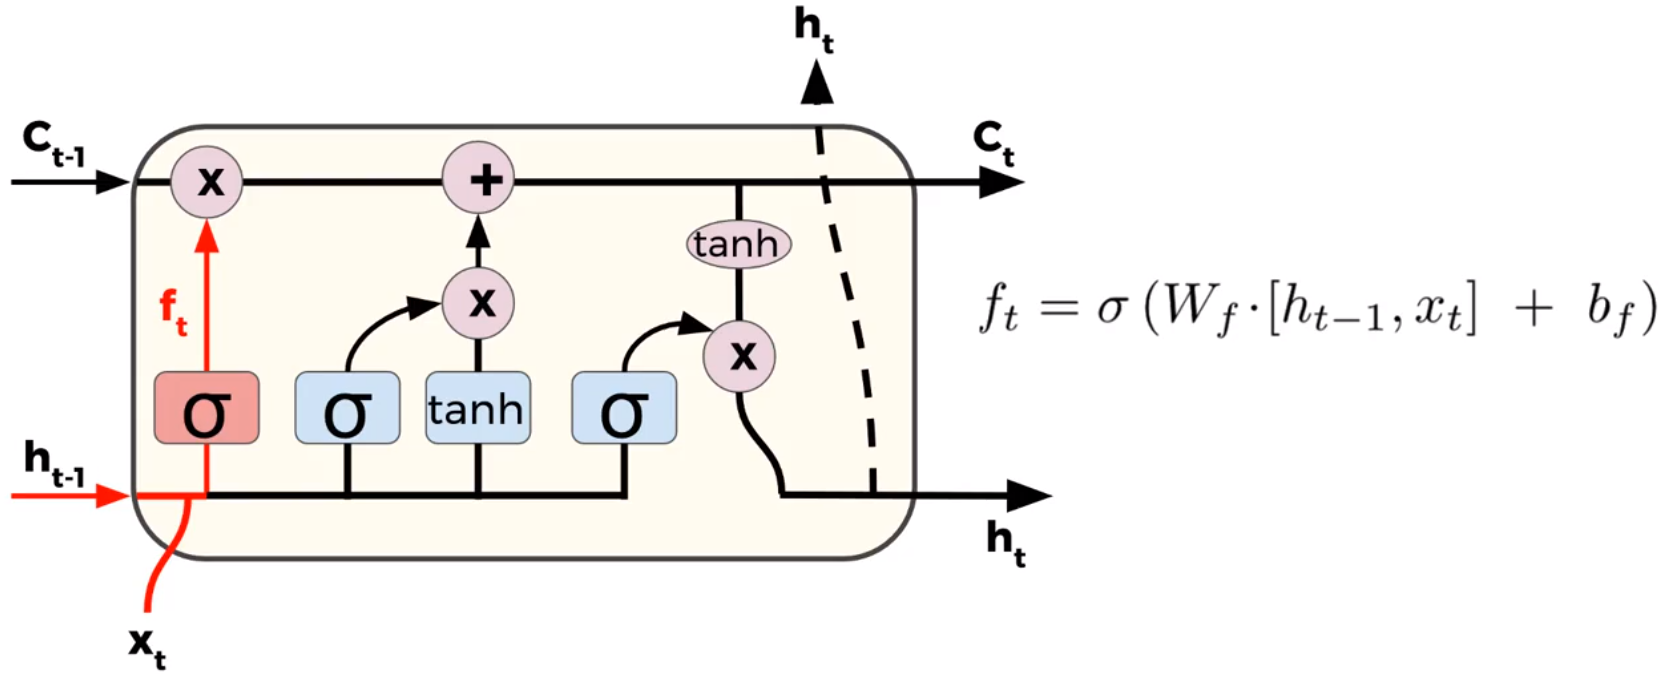
\includegraphics[width=0.7\linewidth]{lstm_forget}
		\caption{Pierwszy krok przepływu informacji przez komórkę LSTM $\pagenote{Jose Portilla, \textit{Complete Guide to TensorFlow for Deep Learning with Python}}$}
		\label{fig:lstmforget}
	\end{figure}
	
	W kolejnym kroku następna bramka decyduje jaką informacje należy zachować. Bramka składa się z dwóch części: funkcji sigmoidalej oraz tanh. W wyniku otrzymywany jest wektor, który jest nazywany wektorem nowych wartości kandydujących
	
	\begin{figure}[H]
		\centering
		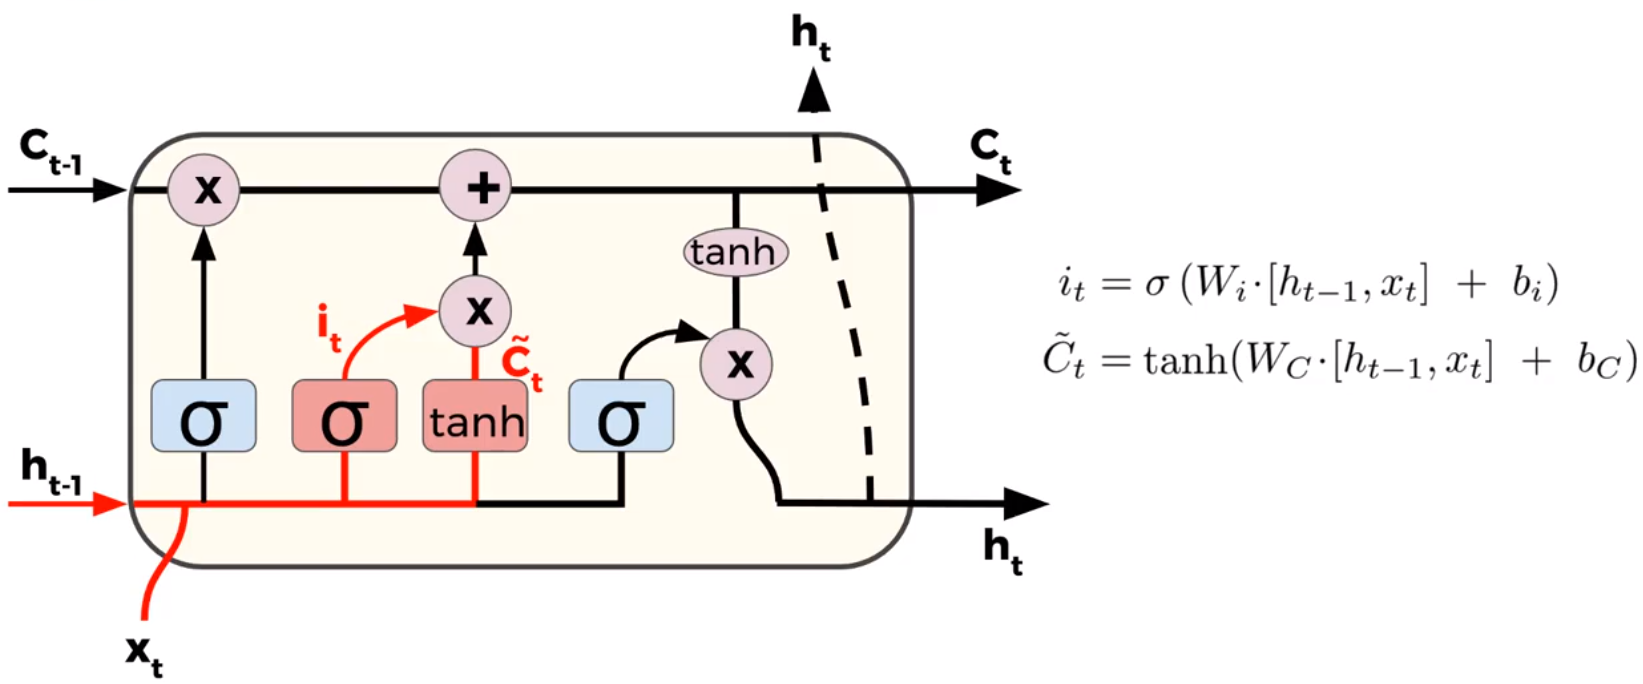
\includegraphics[width=0.7\linewidth]{lstm_2_krok}
		\caption{Drugi krok przepływu informacji przez komórkę LSTM $\pagenote{Jose Portilla, \textit{Complete Guide to TensorFlow for Deep Learning with Python}}$}
		\label{fig:lstm2krok}
	\end{figure}

	W kolejnym kroku następuje aktualizacja starego stanu komórki, który jest określony przez $c^{t-1}$. Zaktualizowany wektor $c^{t}$ jest odbierany przez kolejną komórkę LSTM w kolejnym kroku czasowym.

	\begin{figure}[H]
		\centering
		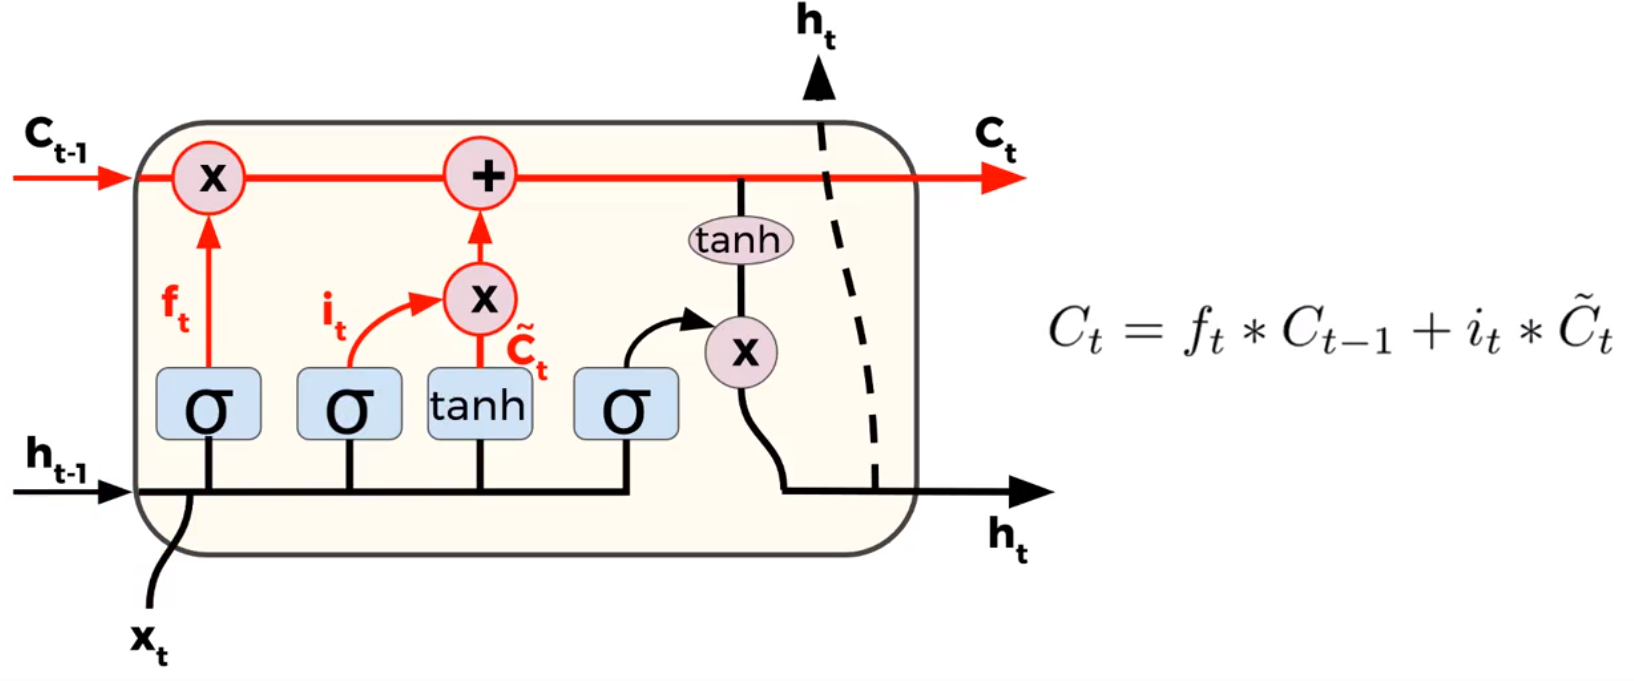
\includegraphics[width=0.7\linewidth]{lstm_3_krok}
		\caption{Trzeci krok przepływu informacji przez komórkę LSTM $\pagenote{Jose Portilla, \textit{Complete Guide to TensorFlow for Deep Learning with Python}}$}
		\label{fig:lstm3krok}
	\end{figure}

	Ostatni krok do zwrócenie wartości $h^{t}$, wartość $h^{t}$ jest wartością przewidywaną przez komórkę LSTM w czasie $t$. Połączenie skierowane do góry może posłużyć jako wejście do kolejnej warstwy ukrytej, znajdującej się bezpośrednio nad aktualną. Połączenie skierowane w prawo, stanowi wejście do następnej komórki LSTM.

	\begin{figure}[H]
		\centering
		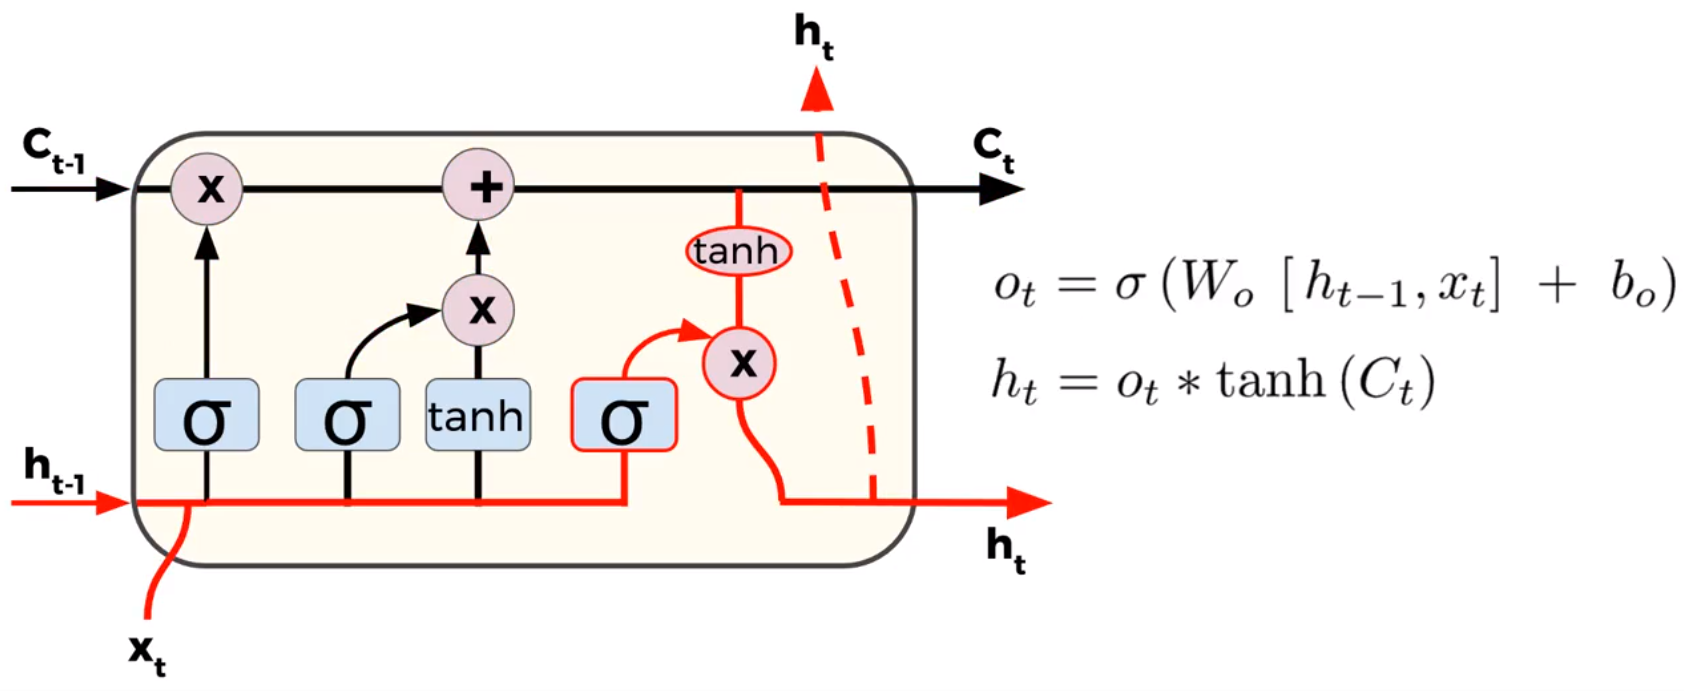
\includegraphics[width=0.7\linewidth]{lstm_4_krok}
		\caption{Czwarty, ostatni krok przepływu przez komórkę LSTM $\pagenote{Jose Portilla, \textit{Complete Guide to TensorFlow for Deep Learning with Python}}$}
		\label{fig:lstm4krok}
	\end{figure}
	
	Badania wykazują, że sieci LSTM znacznie szybkiej przychodzi poznawanie długotrwałych zależności, przede wszystkim na sztucznych zbiorach danych, zaprojektowanych do testowania takich możliwości (Bengio et al., 1994; Hochreiter and Schmidhuber, 1997; Hochreiter et al., 2001). Testy odbywają się na specjalnych wymagających zadaniach przetwarzania sekwencji (Graves, 2012	Graves et al., 2013; Sutskever et al., 2014).
	Nie wszystkie warianty komórek LSTM są takie same jak opisane powyżej. W publikacjach opisujących LSTM można znaleźć wiele innych wariantów, które są lekko odbiegają od oryginalnego modelu. Jednym z popularnych odmian LSTM jest dodatek wprowadzony przez Gersa i Schmidhubera (2000), który wzbogaca standardową komórkę LSTM o tzw. peephole connections. Są to dodatkowe połączenia pomiędzy stanem pamięci, a bramkami. Nieco innym wariantem LSTM jest Gated Recurrent Unit (GRU), koncept ten został wprowadzony przez Cho, et al (2014)$\pagenote{\texttt{http://arxiv.org/pdf/1406.1078v3.pdf}}$. Jednostka GRU łączy bramkę zapomnienia oraz bramkę aktualizacji. Połączony jest także stan komórki ze stanem ukrytym. Uzyskany model jest prostszy niż standardowe modele LSTM i jest coraz bardziej popularny. Inne popularne modele to Depth Gated RNNs authorstwa Yao, et al (2015). Zupełnie inne podejście przedstawił Koutnik w 2014 w pracy Clockwork RNN. Greff, et al. (2015) zrobił porównanie wszystkich popularnych wariantów i stwierdził, że wszystkie działają tak samo. Rafał Józefowicz$\pagenote{\texttt{http://proceedings.mlr.press/v37/jozefowicz15.pdf}}$ przetestował ponad dziesięć tysięcy różnych architektur i wskazał, że niektóre z nich działają lepiej od standardowej komórki LSTM w zależności od postawionego problemu. 
	
	\subsection{Rodzaj sieci "Sequence to sequence"}
	
	Modele sekwencyjno-sekwencyjne (seq2seq) (Sutskever i in., 2014, Cho i in., 2014)$\pagenote{\texttt{https://papers.nips.cc/paper/5346-sequence-to-sequence-learning-with-neural-networks.pdf}}$ odniosły bardzo duży sukces w modelowaniu zadań dla rekurencyjnych sieci neuronowych takich jak tłumaczenie tekstu, rozpoznawanie mowy czy synteza tekstu. Starsze systemy tłumaczenia tekstu rozbijały zdanie na słowa i dokonywały tłumaczenia pojedynczych wyrazów bez zachowania kontekstu zdania. W modelu seq2seq jest przetwarzana cała sekwencja wejściowa i dopiero na podstawie jej kontekstu jest produkowane wyjście. W skład takiego modelu wchodzi mechanizm odpowiedzialny za kodowanie i dekodowanie sekwencji.
	
	\begin{figure}[H]
		\centering
		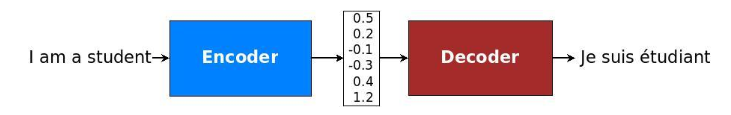
\includegraphics[width=0.7\linewidth]{encoder_decoder}
		\caption{Architektura enkoder - dekoder. Enkoder odpowiedzialny jest za konwersje zdania źródłowego na wektor "znaczeniowy", który jest przekazywany przez dekoder w celu procesu tłumaczenia.$\pagenote{\texttt{https://github.com/tensorflow/nmt}}$ }
		\label{fig:encoderdecoder}
	\end{figure}

	\begin{figure}[H]
		\centering
		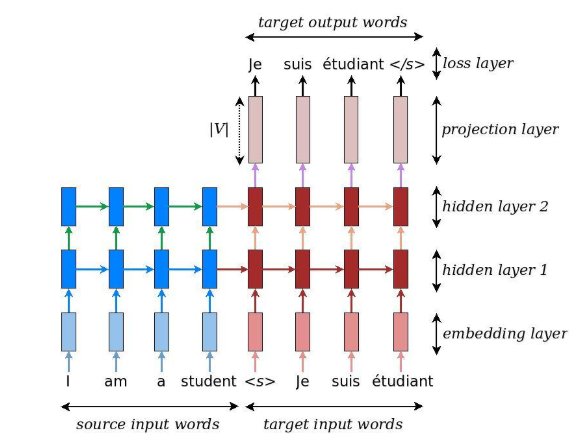
\includegraphics[width=0.8\linewidth]{seq2seq3}
		\caption{Przykład architektury enkoder-dekoder, której zadaniem jest przetłumaczenie zdania "I am a student" na język francuski "Je suis étudiant". Specjalny znacznik "$<s>$" oznacza rozpoczęcie dekodowania, "$</s>$" oznacza zatrzymanie dekodowania. $\pagenote{\texttt{https://github.com/tensorflow/nmt}}$ }
		\label{fig:seq2seq3}
	\end{figure}
	\begin{figure}[H]
		\centering
		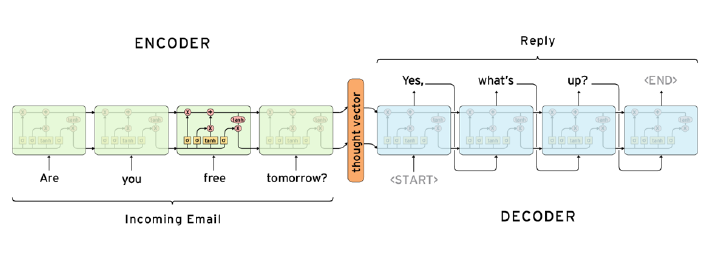
\includegraphics[width=0.8\linewidth]{seq2seq2}
		\caption{Inny przykład architektury seq2se2 zastosowanej do automatycznej odpowiedzi na wiadomości e-mail}
		\label{fig:seq2seq2}
	\end{figure}		
	Muzyka oparta jest na sekwencjach, gdzie kolejny zestaw sekwencji do odegrania zależy od poprzedniego zestawu sekwencji. Model seq2seq może zostać wykorzystany z powodzeniem do wygenerowania nut na podstawie nauczonych sekwencji.	
	\subsection{Rodzaj sieci "Character RNN"}
	Jednym z przykładów sieci operującej bezpośrednio na znakach jest model Character RNN, który został opracowany przez Andreja Karpathego$\pagenote{\texttt{http://karpathy.github.io/2015/05/21/rnn-effectiveness/}}$. Zadaniem sieci po wytrenowaniu jest przewidywanie następnego znaku biorąc pod uwagę sekwencję poprzednich znaków. Taki model można zastosować do generowania muzyki pod warunkiem, że dane wejściowe będą zapisane w formacie tekstowym. Jednak w przeciwieństwie do modelu seq2seq character rnn nie jest w stanie zachować dłużej frazy, ponieważ operuje bezpośrednio na znakach, a nie na sekwencjach. Schemat działania modelu został zilustrowany poniżej.
	
	\begin{figure}[H]
		\centering
		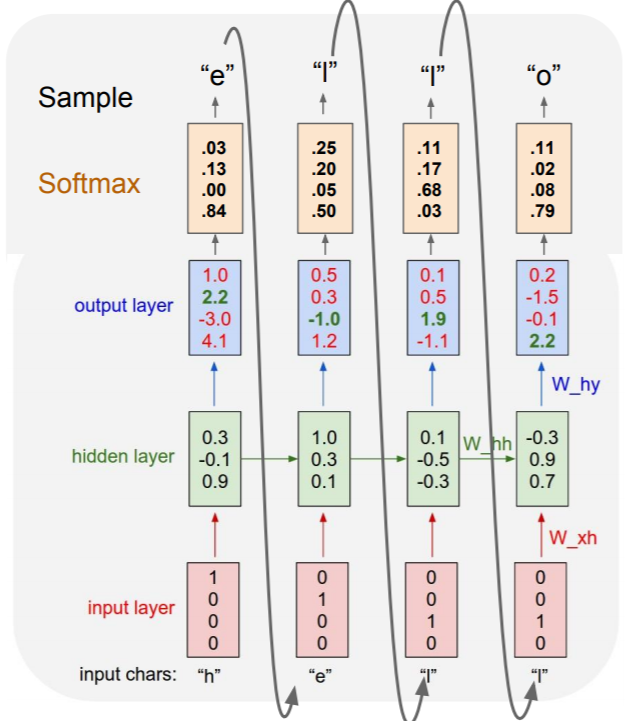
\includegraphics[width=0.5\linewidth]{char_rnn}
		\caption{Schemat modelu Char RNN $\pagenote{\texttt{http://cs231n.stanford.edu/slides/2017/cs231n\_2017\_lecture10.pdf}}$}
		\label{fig:charrnn}
	\end{figure}
	
	Rysunek powyżej ilustruje przykład, w którym rekurencyjna sieć neuronowa uczy się następstwa znaków w wyrazie $\textit{hello}$. Każdy ze znaków jest kodowany za pomocą metody one hot encoding$\pagenote{\texttt{https://machinelearningmastery.com/why-one-hot-encode-data-in-machine-learning/}}$. W pierwszym kroku czasowym dla znaku h zostało przypisane zaufanie wynoszące 1.0, dla kolejnej litery h zaufanie wynosi 2.2, dla e -3.0 oraz l 4.1. W wyrazie hello po literze h występuje litera e, więc sieć powinna zwiększyć zaufanie do tej litery i zmniejszyć do innych. Aby obliczyć w którym kierunku dostosować wagi dla każdej z liter stosuje się algorytm propagacji wstecznej. Cały proces powtarzamy dopóki prognozy sieci będą zgodne z danymi treningowymi. Model ten można przedstawić jako pewne zadanie klasyfikacji, w którym klasy wyników są znakami. Niech $y$ będzie wektorem, który reprezentuje jeden znak zakodowany za pomocą metody one hot encoding. Wektor prawdopodobieństw wystąpienia kolejnego znaku oznaczmy przez $\hat{y}$ to błąd dla pojedynczego znaku można zdefiniować za pomocą $- \sum_{i=0}^{n} y_{i} log(\hat{y_{i}})$.



	\subsection{Metody regularyzacji}	

	Jednym z problemów w systemach uczących się jest sposób zaprojektowania algorytmu, który będzie działać poprawnie nie tylko na danych treningowych, ale także na nowych danych wejściowych. Problem związany z uczeniem polega na tym, że w trakcie uczenia nie jest minimalizowany oczekiwany błąd sieci, ale oczekiwany błąd wyznaczony dla zbioru uczącego. Najbardziej pożądaną cechą systemów uczących jest zdolność algorytmu do generalizacji zdobytej wiedz na nowe przypadki. Dlatego naturalną rzeczą jest dzielenie danych na zbiór testowy i treningowy. 

	Głównym problemem w systemach uczących się jest sposób zaprojektowania algorytmu, który będzie działać dobrze nie tylko na danych treningowych, ale także na nowych danych wejściowych. Zasadniczym problemem związanym z podejściem skrótowo przedstawionym powyżej jest to, że w rzeczywistości w trakcie uczenia nie jest minimalizowany oczekiwany błąd sieci, lecz błąd wyznaczony dla zbioru uczącego. Inaczej mówiąc, najbardziej pożądaną cechą sieci jest jej zdolność do generalizacji swojej wiedzy na nowe przypadki.
	Przejawem przedstawionego rozróżnienia między tym, czego chcielibyśmy uczyć sieć, a tym, czego ją naprawdę uczymy jest problem tak zwanego przeuczenia sieci (problem nadmiernego dopasowania).
	
 	\par
	
	W przypadku głębokiego uczenia regularyzacja jest sposobem na uniknięcie nadmiernego dopasowania. Zadaniem metod regularyzacyjnych jest dodanie tak zwanej kary do funkcji błędu celem zmniejszenia nadmiernego dopasowania. Jedną z metod regularyzacji w sieciach neuronowych jest metoda Dropout$\pagenote{Dropout: a simple way to prevent neural networks from overfitting, Nitish Srivastava and. others, Journal of Machine Learning Research 15.1, pages 1929-1958, 2014, \\\texttt{http://www.jmlr.org/papers/volume15/srivastava14a/srivastava14a.pdf).}}$
	Metoda ta polega na "usuwaniu" z pewnym prawdopodobieństwem poszczególnych neuronów. Usuwanie jednostek stosowane jest dla neuronów w ukrytych warstwach sieci w wyższych warstwach sieci. Podczas fazy treningu sieci neuronowej ułamek jednostek ukrytych jest losowo odrzucany przy każdej iteracji z prawdopodobieństwem $p_{drop}$. Prawdopodobieństwo $p_{drop}$ jest w trakcie konstruowania algorytmu. Powszechnym wyborem jest $p_{drop} = 0.5$. W momencie kiedy część neuronów jest dezaktywowana dokonywane jest przeskalowanie wag aby uwzględnić brakujące neurony. Efekt losowego odrzucenia neuronów zmusza sieć do uczenia się nadmiarowej reprezentacji danych. W takim wypadku sieć nie może polegać na aktywacji jakiegokolwiek zbioru ukrytych neuronów, ponieważ mogą one zostać dezaktywowane w dowolnym momencie podczas treningu.
	\begin{figure}[H]
		\centering
		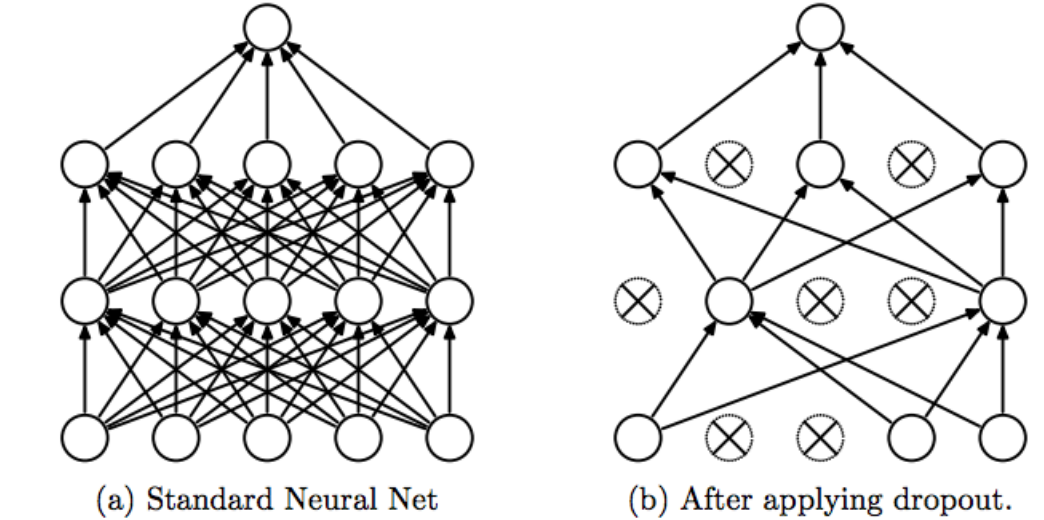
\includegraphics[width=0.7\linewidth]{dropout}
		\caption{Standardowa sieć neuronowa na rysunku po lewej i ta sama sieć po zastosowaniu metody dropout po prawej stronie $\pagenote{Srivastava, Nitish, et al. \textit{Dropout: a simple way to prevent neural networks from overfitting}, JMLR 2014}$ }
		\label{fig:dropout}
	\end{figure}